\section{Gestione delle periferiche}
Le periferiche sono utilizzate dai calcolatori per dialogare con l' esterno.
Vedremo ogni periferica come composta da due elementi:
\begin{itemize}
    \item un controllore: l' elemento direttamente connesso al calcolatore e quello con il quale dialoghiamo direttamente
    \item la periferica: la periferica vera e propria che si interfaccia con il mondo esterno
\end{itemize}
Ci sono periferiche diverse per ogni cosa fattibile, spesso chiamate addirittura trasduttori prendendo il termine dall' elettronica.

La visione tradizionale del calcolatore vede l' esistenza di due spazi di indirizzamento: uno per la memoria ed uno per l'I/O, noi useremo questa visione.
Lo spazio di I/O quindi ci da l' accesso ai registri dei controllori, scrivendo e leggendo questi registri possiamo dare comandi e prelevare risultati, in genere interfacciarci, con le periferiche.

Ogni controllore lo vediamo come composto da 3 registri:
\begin{itemize}
    \item registro di controllo: registro in scrittura che permette al calcolatore di dare i comandi alla periferica
    \item registro di stato: utilizzato dal controllore per rappresentare l' esito del comando imposto dal calcolatore. E' pertanto un registro di sola lettura
    \item registro dati: detto anche buffer, usato per trasmettere dati. Può essere in sola lettura, in sola scrittura o bidirezionale in base al tipo di periferica 
\end{itemize}

\subsection{Sottosistema di I/O}
Abbiamo un modulo del sistema operativo che si occupa di:
\begin{itemize}
    \item definire lo spazio dei nomi con cui identificare i dispositivi: cioè fornire delle interfacce affinché l' utente possa interfacciarsi con queste periferiche in maniera corretta e coerente.
    Questi nomi visibili all' utente devono poi essere tradotti negli identificativi della periferica affinché il sistema operativo possa distinguerli.

    \item Gestire i malfunzionamenti: accorgersi che qualcosa è andato storto ed eventualmente riparare la situazione.
    
    \item Garantire la sincronizzazione tra l' attività di un dispositivo e quella del processo che lo ha attivato.
    
    \item Bufferizzazione: disaccoppiamento temporale e spaziale fra processi e periferiche.
\end{itemize}

\subsubsection{Struttura del sottosistema di I/O}
\begin{figure}[H]
    \centering
    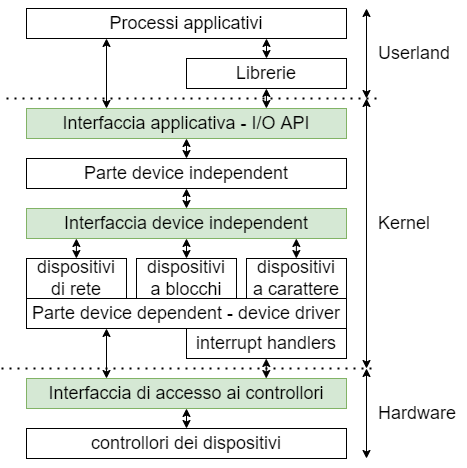
\includegraphics[width=300px]{images/10_Gestione_delle_periferiche/io_subsystem.png}
\end{figure}
Le applicazioni chiamano le primitive del sistema operativo per interfacciarsi con l' I/O, chiamandole direttamente oppure attraverso delle librerie già scritte.
Queste interfacce messe a disposizione dal sistema operativo sono universali e generiche, ad esempio la open, la close, la read, sono primitive generiche usate per qualsiasi dispositivo.

Queste interfacce sono implementate nel sistema di I/O indipendente dal dispositivo, quindi contenente il codice comune a tutte le periferiche.
Ad esempio c'è il codice che si occupa di tradurre il nome del dispositivo usato dall' applicazione nell' ID univoco della periferica.

Il layer device independent a sua volta poggia su alcune interfacce che generalizzano l' accesso alle risorse delle periferiche, queste interfacce sono implementate nei \emph{device driver}, cioè il codice univoco per il tipo di periferica.
Questo codice è l' unico che sa effettivamente come utilizzare i 3 registri che abbiamo elencato sopra.
Una prima divisione tra i dispositivi riguarda la loro tipologia:
\begin{itemize}
    \item dispositivi di rete
    \item dispositivi a blocchi
    \item dispositivi a carattere
\end{itemize}
Il codice del device driver è diviso in due parti:
\begin{itemize}
    \item il codice di gestione
    \item gli interrupt handler
\end{itemize}

\subsection{Funzioni del livello indipendente dai dispositivi}
\subsubsection{Buffering}
Dal momento che noi vogliamo disaccoppiare nel tempo e nello spazio l' utilizzo delle periferiche introduciamo del buffering, questo va eseguito per ogni periferica quindi fa parte della componente device independent.
\begin{figure}[H]
    \centering
    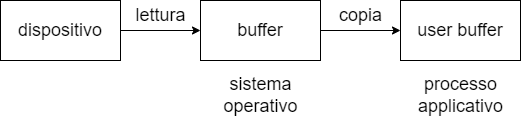
\includegraphics[width=250px]{images/10_Gestione_delle_periferiche/buffering.png}
\end{figure}
Spesso il buffer fornito dall' utente non è il posto migliore per inserire i dati letti dal dispositivo, si ricorre quindi ad un buffer di sistema che è pensato direttamente per gli utilizzi della periferica e non per quelli dell' applicazione.
Per esempio se si volesse leggere un file essendo il disco un dispositivo a blocchi ci serve un buffer grande almeno quanto un blocco, non è detto però che l' utente abbia fornito tutto questo spazio, perché dal canto suo il file è piccolo o vuole leggere solo un certo quantitativo di dati dal file.
Per risolvere il problema disaccoppiamo gli spazi, il blocco lo leggiamo nel buffer del sistema operativo e da qui poi copiamo quanto richiesto nel buffer utente.

Possiamo inventarci strutture più particolari come un doppio buffer per poter accogliere richieste di diversi processi sulla stessa periferica, ad esempio processi diversi che chiedono file diversi.

\subsubsection{Naming}
La traduzione da un nome utilizzabile dall' utente ad un identificativo vero e proprio della periferica è eseguita per tutti i device.

\subsubsection{Gestione dei malfunzionamenti}
Occorre gestire gli errori nelle periferiche, sia direttamente dal sistema operativo (abbiamo copiato male un blocco dal disco ed allora rieseguiamo la copia), sia notificare all' utente affinché possa riparare lui (la carta nella stampante è finita e diciamo all' utente di andare a metterla prima di proseguire).

\subsubsection{Allocazione dei dispositivi ai processi applicativi}
Ogni dispositivo deve essere allocato ai processi che lo richiedono, bisogna quindi gestire l' accesso in modo che sia mutualmente esclusivo e che lasci la periferica in stato consistente.
Non è detto che allocare la periferica in maniera FIFO sia quello più efficiente, possiamo immaginare diversi algoritmi per scegliere l' allocazione.

Bisogna anche controllare che il processo che chiede di utilizzare il dispositivo possa farlo, che ne abbia i privilegi.

\subsection{Funzioni del livello dipendente dai dispositivi}
Questa porzione del modulo si occupa di eseguire le vere e proprie azioni generiche richieste dal layer superiore.
Deve quindi sapere come utilizzare i registri della periferica per arrivare allo scopo.
Supponiamo che il layer superiore richieda:
\begin{verbatim}
    N = read(disp, buffer, nbytes);
\end{verbatim}
in base al valore di disp questa funzione deve eseguire qualcosa di differente.

Il nostro modello generico per il dispositivo è:
\begin{figure}[H]
    \centering
    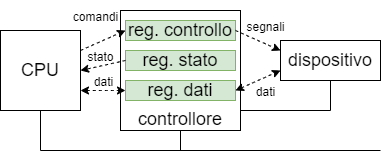
\includegraphics[width=225px]{images/10_Gestione_delle_periferiche/device_logic_scheme.png}
\end{figure}
La CPU inserisce il comando da eseguire nel registro di controllo, il controllore si interfaccia con il dispositivo e gli trasmette il comando.
Il dispositivo una volta finito lo trasmette e trasmette gli eventuali dati prodotti.
Il controllore prende questi dati e li mette a disposizione della CPU insieme al valore dello stato che indica l' esito dell' operazione.

La CPU può conoscere l' esito facendo polling, quindi in una busy-wait controlla il valore del registro di stato, oppure può stopparsi ed aspettare la notifica del controllore tramite una interruzione.

\subsubsection{Processo esterno e processo applicativo}
Dato che nel calcolatore qualsiasi unità di elaborazione appartiene ad un processo creiamo l' astrazione di processo esterno per rappresentare il codice ed i dati che modellano la periferica.

Il processo esterno aspetta che la periferica riceva un comando tramite il registro di controllo.
Aspetta l' esecuzione del comando ed alla fine (denotata da una interruzione) il processo esterno si risveglia e tramite il registro di stato ottiene l'esito del comando.
Alla fine si rimette in attesa di un nuovo comando.

Il processo applicativo invece prepara il comando e lo spedisce alla periferica, dopodiché si mette in attesa del processo esterno.
La periferica esegue ciò che deve fare, risveglia il processo esterno ed il processo esterno risveglia il processo applicativo.

\subsubsection{Astrazione di un dispositivo}
Come prima cosa dobbiamo creare una struttura dati che astragga la periferica, i processi applicativi vi si interfacciano tramite le primitive mentre l' hardware vi si interfaccia tramite l' handler delle interruzioni.
Alcune informazioni da tenere all' interno del descrittore sono:
\begin{itemize}
    \item indirizzo registro di controllo
    \item indirizzo registro di stato
    \item indirizzo registro dei dati
    \item semaforo di sincronizzazione tra il processo applicativo ed il gestore del dispositivo: \verb{dato_disp{
    \item contatore dei dati da trasferire
    \item puntatore al buffer di memoria (di sistema)
    \item esito del trasferimento per l' error handling
\end{itemize}

\subsubsection{Struttura di un device driver}
\begin{verbatim}
    int read(int disp, char* pbuf, int cont){
        // inseriamo le informazioni nel descrittore
        descr[disp].cont = cont
        descr[disp].punt = pbuf
        
        < attivazione del dispositivo >
        // ora il bit di stato è 1
        // ed il processo esterno è sveglio
        
        descr[disp].dato_disp.wait()
        
        if(descr[disp].esito == < codice errore >){
            < gestione dell' errore >
            return -1
        }
        
        return cont - descr[disp].cont
    }
\end{verbatim}
    
\begin{verbatim}
    // Gestore delle interruzioni della periferica
    void inth(){
        char b;
        < legge registro stato controllore >
        
        if(bit_errore == 0){
            b = < legge registro dati controllore >
            descr[disp].punt = b
            descr[disp].punt++
            descr[disp].cont--
            
            if(descr[disp].cont != 0)
                < riattivo dispositivo >
            else{
                descr[disp].esito = < OK >
                < disattivo il dispositivo >
                descr[disp].dato_disp.signal()
            }
        }
        else{
            < routine gestione errore >
            if (< errore non recuperabile >){
                descr[disp].esito = NOT_OK
            }
            descr[disp].dato_disp.signal()
        }
        return
    }
\end{verbatim}

\subsubsection{Flusso di controllo durante un trasferimento}
\begin{verbatim}
    Process P1{
        int n
        int ubufsize = 64
        char ubuf[ubufsize]
        < yadda-yadda >

        n = read(in, ubuf, ubufsize)
    }
\end{verbatim}

\subsubsection{Esempio di gestione del timer}
Usando un singolo timer hardware vogliamo permettere di averne vari virtuali.
La struttura dati che gestisce il timer deve contenere necessariamente:

\begin{figure}[H]
    \centering
    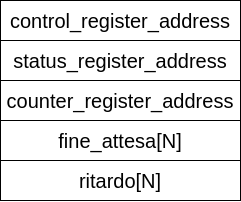
\includegraphics[width=125px]{images/10_Gestione_delle_periferiche/timer_descriptor.png}
\end{figure}

\begin{itemize}
    \item indirizzo del registro di controllo della periferica
    \item indirizzo del registro di stato della periferica
    \item indirizzo del registro contatore della periferica
    \item array dei semafori privati per risvegliare i processi in sleep
    \item array dei ritardi chiesti da ogni processo
\end{itemize}

Scriviamo il codice della primitiva delay() per chiedere di andare in sleep per un certo tempo:
\begin{verbatim}
    void delay(int n){
        int proc
        proc = < indice proc in esecuzione >
        
        descr.ritardo[proc] = n
        descr.fine_attesa[proc].wait()
    }
\end{verbatim}
Il codice dell' interruzione potrebbe essere:    
\begin{verbatim}
    void inth(){
        for(int i = 0; i < N; i++){
            if(descr.ritardo[i] != 0){
                descr.ritardo[i]--
                if(descr.ritardo[i]==0){
                    descr.fine_attesa[i].signal()
                }
            }
        }
    }
\end{verbatim}

\subsubsection{Esempio di gestione dei dischi}
Un disco magnetico è organizzato in dischi, ogni disco è diviso in tracce che sono delle circonferenze formate di un materiale che è capace di mutare il proprio stato magnetico per memorizzare bit.
Il disco ha poi una divisione in settori che sono di fatto dei settori di cerchio quindi possiamo identificare le varie zone in base al numero di traccia ed al numero di settore.

Le tracce più interne del disco sono più dense di informazioni perché più corte mentre quelle più esterne sono meno dense.
Con questa maggiore densità arriva ovviamente un maggiore error rate in lettura.
I gap tra i settori e tra le tracce sono riconoscibili dalla testina che si occupa di leggere il contenuto delle tracce magnetiche oppure di scrivere un valore magnetico su questi blocchi.
All' atto della lettura dobbiamo posizionare la testina su una specifica traccia (in caso di testina mobile) e la rotazione del disco fa si che la traccia scorra e si possano vedere tutti i settori per quella traccia.
Ogni periferica disco ha in realtà più di un disco rotante, spesso si parla infatti di disk pack, ogni singolo layer viene detto cilindro.

Possiamo quindi indicizzare ogni singolo settore tramite numero di cilindro, numero di traccia e numero di settore.
Il tempo medio di trasferimento dipende da diversi fattori come ad esempio:
\begin{itemize}
    \item TA: tempo di accesso cioè il tempo per trovare il settore che si vuole leggere
    \item TT: tempo di trasferimento cioè il tempo che ci vuole per effettuare la vera lettura
    \item RL: rotational latency cioè il tempo che ci mette il disco a ruotare fino a che il settore arrivi sotto la testina
    \item ST: seek time cioè il tempo che ci mette la testina a traslare sulla traccia giusta
\end{itemize}
abbiamo quindi:
$$ TF = TA + TT = ST + RL + TT $$

Se per accedere al disco usiamo la politica FCFS potremmo finire a muovere la testina in maniera poco efficiente ed a farla andare avanti ed indietro in base a come le richieste di lettura vengono fatte al sistema operativo.

Potremmo pensare di utilizzare una tecnica del tipo shortest-seek-time-first cioè una volta eseguito una lettura andare a quella che ha seek time minore di tutti.
Questa tecnica può tuttavia produrre starvation nel caso in cui arrivino regolarmente letture localizzate tutte nella stessa zona e ce ne siano alcune molto lontane.

Un altro algoritmo di scheduling è lo SCAN, si eseguono le letture in maniera ordinata decrescente e successivamente crescente.
In questo modo non abbiamo starvation perché tutte le richieste vengono risolte e chi arriva dopo deve aspettare che la scan sia nella direzione per eseguirla.
Per ricordare la direzione che per adesso stiamo seguendo teniamo in memoria un bit all' interno dello stato della periferica.





